\documentclass[
  journal=,
  manuscript=,
  year=2022,
  volume=01,
]{cup-journal}

\usepackage{amsmath}
\usepackage[nopatch]{microtype}
\usepackage{booktabs}
\usepackage{listings}
\usepackage{xcolor}

\lstset{
    basicstyle          =   \sffamily,          % 基本代码风格
    keywordstyle        =   \bfseries,          % 关键字风格
    commentstyle        =   \rmfamily\itshape,  % 注释的风格,斜体
    stringstyle         =   \ttfamily,  % 字符串风格
    flexiblecolumns,                % 别问为什么,加上这个
    numbers             =   left,   % 行号的位置在左边
    showspaces          =   false,  % 是否显示空格,显示了有点乱,所以不现实了
    numberstyle         =   \zihao{-5}\ttfamily,    % 行号的样式,小五号,tt等宽字体
    showstringspaces    =   false,
    captionpos          =   t,      % 这段代码的名字所呈现的位置,t指的是top上面
    frame               =   lrtb,   % 显示边框
}

\lstdefinestyle{Octave}{
language        =   Octave, % 语言选Python
basicstyle      =   \zihao{-5}\ttfamily,
numberstyle     =   \zihao{-5}\ttfamily,
keywordstyle    =   \color{blue},
keywordstyle    =   [2] \color{teal},
stringstyle     =   \color{magenta},
commentstyle    =   \color{red}\ttfamily,
breaklines      =   true,   % 自动换行,建议不要写太长的行
columns         =   fixed,  % 如果不加这一句,字间距就不固定,很丑,必须加
basewidth       =   0.5em,
}


\usepackage[UTF8]{ctex}
\usepackage{xeCJK}

\title{关于常态化防控核酸检测效率的研究与讨论}

\author{周子钰}
\affiliation{First Division, 山东农业大学, 信息科学与工程学院,计算机类,2022级09班}
\email[周子钰]{JunASAKA@zzy040330.moe}

\author{王兆艳}
\affiliation{Second Division, 山东农业大学, 信息科学与工程学院,计算机类,2022级11班}
% \alsoaffiliation{Joint first authors}

% \author{T. Author}
% \affiliation{Second Division, Organization, City, Pincode, State, Country}

% \author{F.T. Author}
% \affiliation{Fourth Division, Organization, City, Pincode, State, Country}

\addbibresource{ref.bib}

\keywords{TOPSIS, AHP, Normal distribution, Poisson distribution, Monte Carlo method} %% First letter not capped

\begin{document}

\begin{abstract}
\par   集中检测核酸是当前新冠防疫的最主要检测措施和方式;为解决核酸检测效率问题,设计不同数学模型进行分析,并为核酸检测的智能管理提供科学性建议。
\par 本研究采用AHP(Analytic Hierarchy Process)、带权重的TOPSIS(Technique for Order Preference by Similarity to Ideal Solution)、正态分布模型等评价评估方法进行分析,使用开源、自由的科学计算软件Octave进行计算,找出目前影响核酸检测效率主要因素,并针对各因素提出合理的解决方案。
\end{abstract}

% \noindent Lorem ipsum dolor sit amet, consectetur adipiscing elit, sed do eiusmod tempor incididunt ut labore et dolore magna aliqua. 

\section{问题提出}

\par 集中检测核酸是当前新冠防疫的最主要检测措施和方式。但核酸检测点常常出现一种现象:时而队如长龙,时而无人问津。这会导致检测效率下降,浪费了医务人员和人们的宝贵时间,且增加了传染的风险,为研究如何让人们科学有效地完成核酸检测,问题由此产生。

\begin{enumerate}
    \item 分析确定合理的评价体系,评估当前核酸检测站点的总体效率,并找出影响效率的问题所在。
    \item 针对问题一的分析结果,经过恰当地计算、分析、评估,给出合理的意见和建议以解决对应的问题。
    \item 应用统计学、数学、计算科学等方法为该参检用户提出合理的参与核酸检测有关的建议。
\end{enumerate}

\section{符号说明与模型假设}

\par 符号说明:

\begin{enumerate}
	\item $X_{i}$:评价指标。
	\item $x_{ij}$:数据矩阵中的一个元素。
	\item $z_{ij}$:标准化后的元素。
	\item $D_{i}$:欧氏距离。
	\item $\overrightarrow{W}$, $\overrightarrow{w}$:权向量。
	\item $\bar{C}$:加权平均值。
	\item $\xi$:随机变量。
	\item $\alpha$:置信度。
\end{enumerate}

\par 基本假设:

\begin{enumerate}
	\item 可能参与核酸检测的人员无限。
	\item 数据来源于调查问卷、实地考察、手动测量等途径,真实可靠。
	\item 核酸检测时单位时间内到达的人数服从泊松分布(Poisson distribution),且在两个不相交时间段内人员到达情况相互独立。
	\item 不考虑设备故障、极端天气等特殊状况对实验的影响。
\end{enumerate}

\section{模型建立与模型求解}

\subsection{核酸检测现状分析}

\par 以青岛市某小区正门门口的核酸检测点为调查对象。该核酸检测点有三个检测窗口,通常开放时间为日间7时至11时半、午后二时至晚间六时半,全天共开放九小时。该站点周围居民密度大且流动性较大,约有8000-10000人:其中,在此参加核酸检测的居民约五千人许。该站点支持三种人员登记技术,分别为:以近场通信(Near Field Communication)为主的RFID(Radio Frequency Identification)无线电射频识别技术、QR Code(クイック-レスポンス コード) 高速反馈矩阵式二维码解码识别技术,以及用键盘人工录入参检人员信息。其中,近场RFID射频技术仅有窗口三支持,QR Code技术仅窗口一和窗口二支持,同时,三个窗口都接受手动录入的方式。
\par 调查显示,大众对三种登记方式的偏好不同。例如,年轻人偏好使用QR Code技术登记,而老年人常常由于仅持有性能有限的移动终端,无法快速地启动、展示自己的QR Code,而偏好使用RFID射频技术进行识别认证,对于部分未成年人,其尚未办理二代身份证或不方便使用QR Code,仅可使用手动登记的方式录入信息。
\par 经统计,2022年10月25日,所述三种方式使用人数占比如图一所示。

\begin{figure}[hbt!]
	\centering
	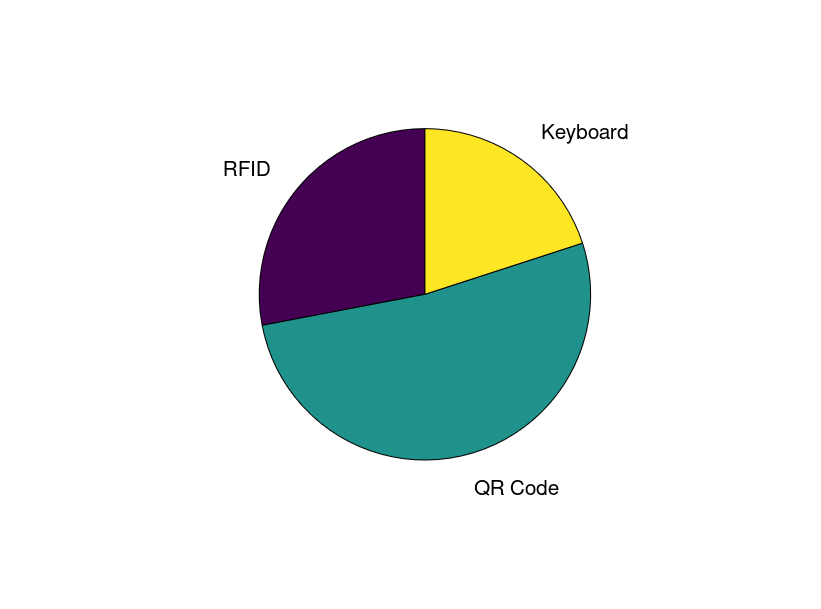
\includegraphics[width=0.75\linewidth]{fig/r.png}
	\caption{登记方式占比}
	\label{fig_rec}
\end{figure}

\par 由统计图可以看出,偏好QR Code登记方式的用户占多数,而偏好RFID与手动录入的用户各占约1/4,其中偏好RFID的用户相对较多。
\par 由于目前核酸检测规定为“三天两检”,固然会出现不同日期内核酸检测人数差异较大。
\par 此处暂不考虑“三天两检”对实验的影响,为避免出现系统性的误差。为科学有效建立模型,使该模型更加广泛的应用,为人们核酸检测提供便利,图二给出一周内(2022年10月23-29日)每天午前九时时的核酸检测排队人数的;该数据为完全统计量,真实可靠。

\begin{figure}[hbt!]
	\centering
	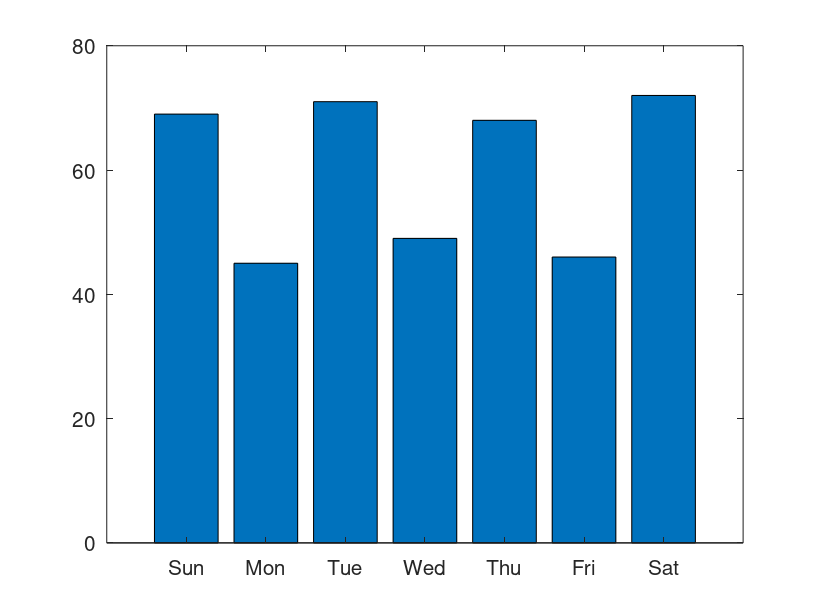
\includegraphics[width=0.75\linewidth]{fig/n.png}
	\caption{不同时间的人数变化}
	\label{fig_num}
\end{figure}

\par 在采样日内,人数变化较大,从图表统计可以看出人数分布不均匀,但差距较小。说明居民对核酸检测需求较大且稳定。但调查数据显示每日内不同时段,人数变化极大,效率不稳定。

\par 为评估该站点检测效率,统计共计2287人的排队时间,以下为随机挑选的100组数据。

\begin{figure}[hbt!]
	\centering
	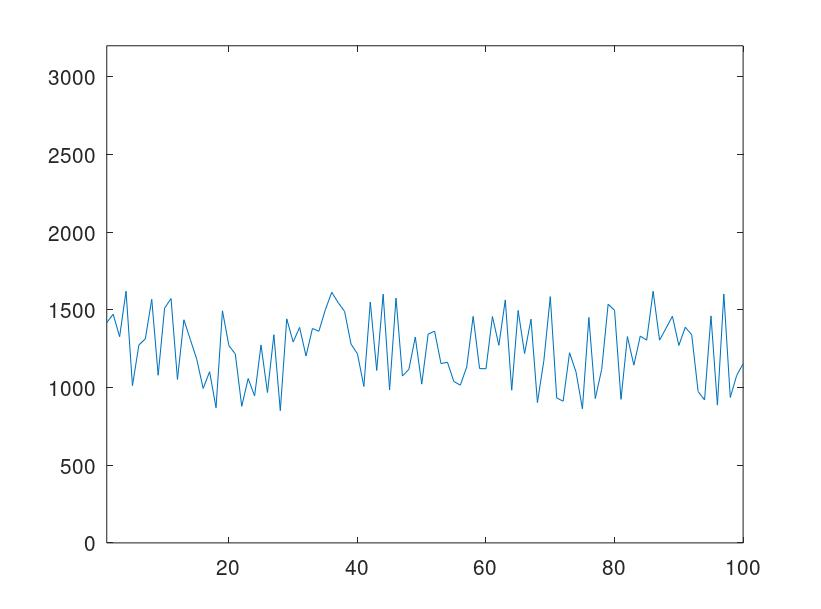
\includegraphics[width=0.75\linewidth]{fig/t.jpg}
	\caption{排队时间}
	\label{fig_time}
\end{figure}

\par 从随机理论上来说,单位时间内到达检测站点的人数服从泊松分布,而参检人员到达检测站点后接受检测的时间是一个相当固定的常数;由图三及所有统计数据得知,该站点排队时间基本分布在x区间内,且相对均匀,倘若将该随机时间看作随机变量,那么该随机变量近似可以认为是一种均匀分布。

\subsection{Model 1 带权重的类TOPSIS评价评估模型}
\noindent 参引文献:\cite{chakraborty2022topsis}。Octave程式代码见Appendix 1。
\par 核酸检测的总过程分为两个步骤:等级、采样;此前由于参检人数多,通常需要排队等待检测。其中,正如上文所述,采样步骤共有三种可选的采样方式:近场无线电射频技术、高速反馈二维矩阵码识别技术、手动录入个人信息,此三种等级方式在不同窗口的支援情况不同,且由于技术原因,其等级所消耗的时间不同,此些问题接纳入考量范围。显而易见地,核酸检测站点的工作效率、工作效率主要体现在“平均排队时间”、“平均登记时间”、“平均采样时间”;这三种“时间”越短反映了核酸检测效率越高。此外,该站点共有三个不同的核酸检测窗口,而开放的窗口数对核酸检测的效率也有着直接的且较大的影响。
\par 在我们实验调查中,人们在等待时大多遵纪,极少出现混乱,且会提早为检测需要的材料做准备,在此受检测者的因素暂且可以忽略。
\par 考虑以上因素,在对当前核酸检测站点进行效率评估时,应重点考察如下指标:开放的窗口数、平均排队时间、平均登记时间、平均采样时间。
\par 目前对指标优劣评价的模型有很多,如AHP(Analytic Hierarchy Process)多方案决策法、Synthetical Index Method、RSR(Rank-Sum Ratio)法、Grey System灰色系统法、Fuzzy Comprehensive Evaluation Method等,这些各自具有不同的特点,对不同问题的解决各有利弊。其中,TOPSIS 综合评价法是系统中“有限方案多目标”决策分析中的一种决策方法。其计算简便,结果合理,应用较为灵活;配合多种计算评价指标权重的方法,适合于解决此问题。
\par 下面根据原始数据,利用TOPSIS(Technique for Order Preference by Similarity to Ideal Solution)理想逼近解排序法来评估当前运作形式下该核酸检测站点的工作效率。

\subsubsection{指标分类、代号与权重}

\par 经过实地咨询,核酸检测志愿者对评估的各项指标进行筛选,并与社会学家交流后,对筛选后的各个指标进行评估,使用专家估计法最终得出权重。

\begin{table}[hbt!]
	\begin{threeparttable}
	\caption{各评价指标属性}
	\label{table_1}
	\begin{tabular}{llll}
	\toprule
	\headrow 指标 & 权重 & 代号 & 类型 \\
	\midrule
	窗口数(个) & 0.4 & $X_{0}$ & 极大型 \\
	\midrule
	平均排队时间(秒) & 0.15 & $X_{1}$ & 极小型 \\
	\midrule
	平均登记时间(秒) & 0.3 & $X_{2}$ & 极小型 \\
	\midrule
	平均采样时间(秒) & 0.15 & $X_{3}$ & 极小型 \\
	\bottomrule
	\end{tabular}
	\end{threeparttable}
\end{table}

\subsubsection{统计数据表}

\par 根据现场观察,不同窗口之前排队的人数基本一致,且每个窗口的志愿者进行采样时采用的具体方法唯一,故排队时间与采样时间取多次测量结果的平均值进行分析。

\begin{table}[hbt!]
	\begin{threeparttable}
	\caption{各录入方式的各项评价指标数据}
	\label{table_2}
	\begin{tabular}{lllll}
	\toprule
	\headrow  & $X_{0}$ & $X_{1}$ & $X_{2}$ & $X_{3}$ \\
	\midrule
	RFID & 1 & 1560 & 3.6 & 3.7 \\
	\midrule
	QR Code & 2 & 1560 & 6.2 & 3.7 \\
	\midrule
	手动输入 & 3 & 1560 & 15 & 3.7 \\
	\bottomrule
	\end{tabular}
	\end{threeparttable}
\end{table}


\subsubsection{权向量确定}

\par 通过与社会学家交流,对筛选后的各个指标进行评估,使用专家估计法最终得出权重向量为:

\begin{equation}
	\begin{aligned}
		\overrightarrow{W}=
		\begin{bmatrix}
			0.4 & 0.15 & 0.3 & 0.15
		\end{bmatrix}
	\end{aligned}
\end{equation}

\subsubsection{指标的正向化(同趋势化)处理。}

\par 原始数据中,“窗口数”越大越好,为极大型数据,而“平均排队时间”、“平均登记时间”、“平均采样时间”越小越好,为极小型数据。为将所有不同类型的指标统一为极大型指标,故对所有极小型指标采用用差值法$(1–X_{i})$进行转换。
\par 转换后得到的数据矩阵:

\begin{equation}
	\begin{aligned}
		X=
		\begin{bmatrix}
			1 & 1560 & 11.4 & 3.7 \\
			2 & 1560 & 8.8 & 3.7 \\
			3 & 1560 & 0 & 3.7
		\end{bmatrix}
	\end{aligned}
\end{equation}

\subsubsection{数据的标准化(Standardization)与归一化(Normalization)}

\par 为了消除不同量纲对评价结果的影响, 使评价的多指标在同一个量纲体系下进行比较, 需对原始数据进行规一化处理。处理的方法为:

\begin{equation}
	\begin{aligned}
		z_{ij}=\frac{x_{ij}}{\sqrt{\sum_{i=1}^{n} x_{ij}^{2} } }
	\end{aligned}
\end{equation}

\par 得到的标准化后的数据矩阵为:

\begin{equation}
	\begin{aligned}
		X=
		\begin{bmatrix}
			0.2673 & 0.5774 & 0.7916 & 0.5774 \\
			0.5345 & 0.5774 & 0.6111 & 0.5774 \\
			0.8018 & 0.5774 & 0 & 0.5774
		\end{bmatrix}
	\end{aligned}
\end{equation}

\subsubsection{确定最优向量$Z^{+}$和最劣向量$Z^{-}$,其中为$Z^{+}$同一评价指标的最大归一化值,而$Z^{-}$为同一评价指标的最小归一化值。}

\begin{equation}
	\begin{aligned}
		& \overrightarrow{Z^{+}}=\begin{bmatrix}
			0.8018 & 0.5774 & 0.7916 & 0.5774
		\end{bmatrix}\\
		& \overrightarrow{Z^{-}}=\begin{bmatrix}
			0.2673 & 0.5774 & 0 & 0.5774
		\end{bmatrix}
	\end{aligned}
\end{equation}

\par 其中,$Z_{j}^{+}=\max_{1\le i \le 5}\{z_{ij}\}$,$Z_{j}^{-}=\min_{1\le i \le 5}\{z_{ij}\}$,$j=1,2,3,4$。

\subsubsection{计算各指标与理想解及负理想解的加权欧几里得距离(Euclidean distance)并归一化(Normalization)并计算加权平均值$\bar{C}$}

\par 归一化(Normalization)后的综合评分$\tilde{S}_{i}=\frac{S_{i}}{\sum_{i=1}^{n}S_{i}}$,其中$S_{i}=\frac{D^{-}_{i}}{D^{+}_{-}+D^{-}_{i}}$。而$D^{+}_{i}$与$D^{-}_{i}$用以下公式计算。

\begin{equation}
	\begin{aligned}
		& D^{+}_{i} = \sqrt{\sum_{j=1}^{m}(Z^{+}_{j}-z_{ij})}\\
		& D^{-}_{i} = \sqrt{\sum_{j=1}^{m}(Z^{-}_{j}-z_{ij})} \\
	\end{aligned}
\end{equation}

\par 归一化后的评分向量为:

\begin{equation}
	\begin{aligned}
		X=
		\begin{bmatrix}
			0.3391 \\
			0.3965 \\
			0.2644
		\end{bmatrix}
	\end{aligned}
\end{equation}

\par 通过实地调查,取每种登记方式使用人数的百分比作为权重。权向量为:

\begin{equation}
	\begin{aligned}
		\overrightarrow{w}=
		\begin{bmatrix}
			0.28 \\
			0.52 \\
			0.2
		\end{bmatrix}
	\end{aligned}
\end{equation}

\par 最后计算所得到的加权平均值:

\begin{equation}
	\begin{aligned}
		\bar{C}=\sum_{i=1}^{3}w_{i}C_{i}=0.3540
	\end{aligned}
\end{equation}

\subsection{Octave运算结果}

\begin{figure}[hbt!]
	\centering
	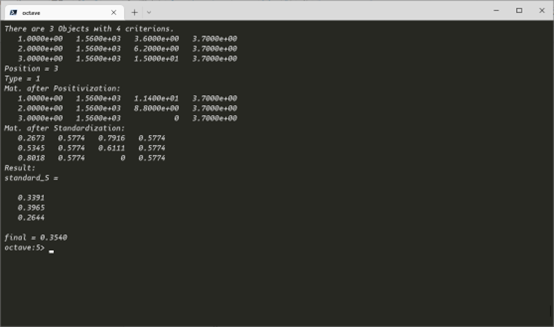
\includegraphics[width=0.75\linewidth]{fig/res1.png}
	\caption{Model 1 Octave运算结果}
	\label{fig_res1}
\end{figure}

\subsubsection{结论}

\par 通过TOPSIS法,我们对原始数据进行了正向指标化(Positivization)、标准化(Standardization)和归一化(Normalization)处理,消除了不同指标的不同量纲对评定的影响。排序的结果充分利用原始数据信息,能定量反映不同评价单元的优劣程度;且较为直观,较为可靠。由于对数据进行归一化(Normalization),该计算所得到的加权平均值,相对接近度值在0 与1 之间。同时,若该值愈接近1,则所评价单元接近最优水平程度愈高;反之,若该值愈接近0,则评价单元接近最优水平的程度愈低或者说愈接近最劣水平。
\par 通过上述的计算与分析,不难发现,该核酸检测点的工作效率较低,相对接近度仅有0.3540。进行深层次分析后可以看出,偏好于使用近场RFID无线电射频登记方法与高速反馈矩阵码的用户较多,而并非所有检测窗口皆兼容这两项技术,这对该核酸检测站点的工作效率有较大的影响。故然,该站点在设备与技术支援方面有较大的改善空间,引进新型设备提高每个登记窗口对不同登记技术的支援度是一个很好的解决方案。
\par 其次,由于登记时间较长,间接造成了排队时间;且由于不同窗口对不同登记方式的支援情况不同,会出现参检人员以更换登记方案的方式来换取较短的排队时间,故然,对不同窗口参检人员的登记方式的规划进行调整,给出用户合理的建议,是一项较为出色的解决方案。由此提出问题2,并引入模型2进行分析、计算与解决。

\subsection{Model 2 基于AHP(Analytic Hierarchy Process)的加权TOPSIS评价模型}
\noindent 参引文献:\cite{vasquez2021ahp}。Octave程式代码见Appendix 2。
\par 按照调查结果,该核酸检测站点支持三种登记方法,分别为:以近场通信(Near Field Communication)为主的RFID(Radio Frequency Identification)无线电射频识别技术、QR Code(クイック-レスポンス コード) 高速反馈矩阵式二维码解码识别技术,以及用键盘人工录入参检人员信息。其中,近场RFID射频技术仅有窗口三支持,QR Code技术仅窗口一和窗口二支持,同时,三个窗口都接受手动录入的方式。
\par 调查显示,大众对三种登记方式的偏好不同。例如,年轻人偏好使用QR Code技术登记,而老年人常常由于仅持有性能有限的移动终端,无法快速地启动、展示自己Code,而偏好使用 RFID射频技术进行识别认证,对于部分未成年人,其尚未办理二代身份证或不方便使用QR Code,仅可使用手动登记的方式录入信息。 


\subsubsection{指标分类、代号与权重}

\par 经过实地咨询,核酸检测志愿者对评估的各项指标进行筛选,并与社会学家交流后,对筛选后的各个指标进行评估,使用AHP(Analytic Hierarchy Process)多方案决策法最终得出各指标的权重。

\begin{table}[hbt!]
	\begin{threeparttable}
	\caption{各评价指标属性}
	\label{table_3}
	\begin{tabular}{llll}
	\toprule
	\headrow 指标 & 权重 & 代号 & 类型 \\
	\midrule
	耗时(秒) & 0.4 & $X_{0}$ & 极小型 \\
	\midrule
	用户偏好(使用人数) & 0.6 & $X_{1}$ & 极大型 \\
	\midrule
	成本(元) & 0.1 & $X_{2}$ & 极小型 \\
	\bottomrule
	\end{tabular}
	\end{threeparttable}
\end{table}

\subsubsection{统计数据表}

\begin{table}[hbt!]
	\begin{threeparttable}
	\caption{各录入方式的各项评价指标数据}
	\label{table_4}
	\begin{tabular}{llll}
	\toprule
	\headrow  & $X_{0}$ & $X_{1}$ & $X_{2}$ \\
	\midrule
	RFID & 3.6 & 0.28 & 79 \\
	\midrule
	QR Code & 6.2 & 0.52 & 259 \\
	\midrule
	手动输入 & 15 & 0.6 & 0.1 \\
	\bottomrule
	\end{tabular}
	\end{threeparttable}
\end{table}


\subsubsection{权向量确定}

\par 通过与社会学家交流,对筛选后的各个指标进行评估,使用专家估计法最终得出权重向量为:

\begin{equation}
	\begin{aligned}
		\overrightarrow{W}=
		\begin{bmatrix}
			0.4 & 0.6 & 0.1
		\end{bmatrix}
	\end{aligned}
\end{equation}

\subsubsection{指标的正向化(同趋势化)处理。}

\par 原始数据中,“用户偏好”越大越好,为极大型数据,而“耗时”、“成本”,为极小型数据。为将所有不同类型的指标统一为极大型指标,故对所有极小型指标采用用差值法$(1–X_{i})$进行转换。
\par 转换后得到的数据矩阵:

\begin{equation}
	\begin{aligned}
		X=
		\begin{bmatrix}
			11.4 & 0.28 & 180 \\
			8.8 & 0.52 & 0 \\
			0 & 0.2 & 259
		\end{bmatrix}
	\end{aligned}
\end{equation}

\subsubsection{数据的标准化(Standardization)与归一化(Normalization)}

\par 为了消除不同量纲对评价结果的影响, 使评价的多指标在同一个量纲体系下进行比较, 需对原始数据进行规一化处理。处理的方法为:

\begin{equation}
	\begin{aligned}
		z_{ij}=\frac{x_{ij}}{\sqrt{\sum_{i=1}^{n} x_{ij}^{2} } }
	\end{aligned}
\end{equation}

\par 得到的标准化后的数据矩阵为:

\begin{equation}
	\begin{aligned}
		X=
		\begin{bmatrix}
			0.7916 & 0.4491 & 0.5707 \\
			0.6111 & 0.8340 & 0 \\
			0 & 0.3208 & 0.8212
		\end{bmatrix}
	\end{aligned}
\end{equation}

\subsubsection{确定最优向量$Z^{+}$和最劣向量$Z^{-}$,其中为$Z^{+}$同一评价指标的最大归一化值,而$Z^{-}$为同一评价指标的最小归一化值。}

\begin{equation}
	\begin{aligned}
		& \overrightarrow{Z^{+}}=\begin{bmatrix}
			0.7916 & 0.8340 & 0.8212
		\end{bmatrix}\\
		& \overrightarrow{Z^{-}}=\begin{bmatrix}
			0 & 0.3208 & 0
		\end{bmatrix}
	\end{aligned}
\end{equation}

\par 其中,$Z_{j}^{+}=\max_{1\le i \le 5}\{z_{ij}\}$,$Z_{j}^{-}=\min_{1\le i \le 5}\{z_{ij}\}$,$j=1,2,3,4$。

\subsubsection{计算各指标与理想解及负理想解的加权欧几里得距离(Euclidean distance)并归一化(Normalization)并计算加权平均值$\bar{C}$}

\par 归一化(Normalization)后的综合评分$\tilde{S}_{i}=\frac{S_{i}}{\sum_{i=1}^{n}S_{i}}$,其中$S_{i}=\frac{D^{-}_{i}}{D^{+}_{-}+D^{-}_{i}}$。而$D^{+}_{i}$与$D^{-}_{i}$用以下公式计算。

\begin{equation}
	\begin{aligned}
		& D^{+}_{i} = \sqrt{\sum_{j=1}^{m}(Z^{+}_{j}-z_{ij})} \\
		& D^{-}_{i} = \sqrt{\sum_{j=1}^{m}(Z^{-}_{j}-z_{ij})} \\
	\end{aligned}
\end{equation}

\par 归一化后的评分向量为:

\begin{equation}
	\begin{aligned}
		\overrightarrow{X}=
		\begin{bmatrix}
			0.4091 \\
			0.4064 \\
			0.1845
		\end{bmatrix}
	\end{aligned}
\end{equation}

\subsection{Octave运算结果}

\begin{figure}[hbt!]
	\centering
	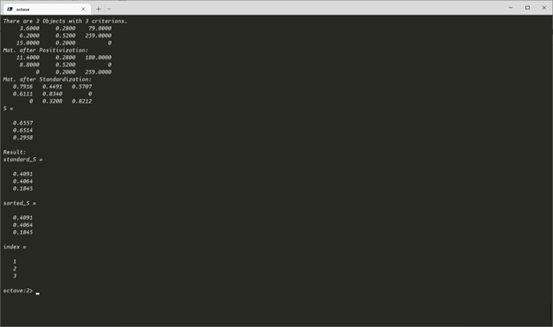
\includegraphics[width=0.75\linewidth]{fig/res2.png}
	\caption{Model 2 Octave运算结果}
	\label{fig_res2}
\end{figure}

\subsubsection{结论}

\par 通过TOPSIS法,我们对原始数据进行了正向指标化(Positivization)、标准化(Standardization)和归一化(Normalization)处理,消除了不同指标的不同量纲对评定的影响。排序的结果充分利用原始数据信息,能定量反映不同评价单元的优劣程度;且较为直观,较为可靠。由于对数据进行归一化(Normalization),该计算所得到的加权平均值,相对接近度值在0 与1 之间。同时,若该值愈接近1,则所评价单元接近最优水平程度愈高;反之,若该值愈接近0,则评价单元接近最优水平的程度愈低或者说愈接近最劣水平。
\par 由原始数据以及计算结果可以看出,三种登记方式各有优劣;综合来说,近场RFID射频技术优于QR Code解码技术,优于手动录入。而偏好于QR Code方式的参检人数较多,应根据上述结果合理调整窗口、设备与工作人员,实现多种登记技术共同高效使用的效果,以提高工作效率。同时,根据前文分析的结果,应在不同时间段内采取不同的管理方式以取得更高的检测效率。

\subsection{Model 3 核酸检测等待时间区间估计模型}
\noindent 参引文献:\cite{yu2014improved}。
\par 按照随机理论来说,单位时间到达核酸检测站点的人数符合泊松分布,而相对于排队时间来说,不同窗口、不同时间内参检人员接受登记与采样的时间相当于一个固定的常数;自原始统计数据可以看出,核酸检测参检排队等待时间基本维持在$\left [ 850,1600 \right ] $的区间内,且相对稳定。此时,倘若将该随机时间看作随机变量,则该分布可以认为是一种均匀分布。

\par 将调查所得的共计2287人的排队时间数据作为样本,排队时间随机变量$\xi_{i}$服从均匀分布,其均值$\xi=\frac{1}{2287}\sum_{i}\xi_{i}$依据大数定律服从正态分布,可以对其正态化以后的统计量进行给定置信度的置信区间估计。

\begin{equation}
	\begin{aligned}
		& \xi=\frac{1}{2287}\sum_{i}\xi_{i} \sim N \left ( \mu, \sigma \right ) \\ \\
		& \Longrightarrow \frac{\xi-E_{\xi}}{\sqrt{D_{\xi}}} \sim N \left ( 0,1 \right ) \\ \\
		& \Longrightarrow P \left ( \left | \frac{\xi-E_{\xi}}{\sqrt{D_{\xi}}} \right | < u_{\frac{\alpha}{2}} \right ) = 1-\alpha \\
	\end{aligned}
\end{equation}

\par 得到置信区间:

\begin{equation}
	\begin{aligned}
		\left ( \xi - u_{\frac{\alpha}{2}} \sqrt{D_{\xi}} , \xi + u_{\frac{\alpha}{2}} \sqrt{D_{\xi}} \right )
	\end{aligned}
\end{equation}

\par 给定置信度 0.95,即$\alpha=0.05$,置信区间为:$\left ( 1019.1,1449.1 \right )$。区间中点$1234.1$表示平均等待登记采样时间。

\section{结论与研究方向}

\par 进行核酸检测已经成为居民生活中不可或缺的一部分,但核酸检测效率直接影响居民和医务人员所耗时间,人数在不同时段分布的巨大差异,增加了人们感染病毒的风险,为疫情防控增加负担,为使居民科学有效地进行核酸检测,我们通过建模设计为居民进行核酸检测时间进行智能推荐,在该模型的应用下,智能推荐核酸检测时间初具雏形。

\begin{acknowledgement}

	This article is using the Template "Cambridge Medium Template Class File" which released under Creative Commons CC BY 4.0 Licence and whose authors are Cambridge University Press and Overleaf. 

This article was released under Creative Commons CC BY 4.0 Licence as well. 

\end{acknowledgement}

\printbibliography

\appendix

\section{Model 1 代码}
\noindent Inter2Max.m:\\
\lstinputlisting[style=Octave]{octave_src/Model1/inter2Max.m}
\noindent main.m:\\
\lstinputlisting[style=Octave]{octave_src/Model1/main.m}
\noindent Mid2Max.m:\\
\lstinputlisting[style=Octave]{octave_src/Model1/mid2Max.m}
\noindent Min2Max.m:\\
\lstinputlisting[style=Octave]{octave_src/Model1/min2Max.m}
\noindent Positivization.m:\\
\lstinputlisting[style=Octave]{octave_src/Model1/positivization.m}

\section{Model 2 代码}
\noindent Inter2Max.m:\\
\lstinputlisting[style=Octave]{octave_src/Model2/inter2Max.m}
\noindent main.m:\\
\lstinputlisting[style=Octave]{octave_src/Model2/main.m}
\noindent Mid2Max.m:\\
\lstinputlisting[style=Octave]{octave_src/Model2/mid2Max.m}
\noindent Min2Max.m:\\
\lstinputlisting[style=Octave]{octave_src/Model2/min2Max.m}
\noindent Positivization.m:\\
\lstinputlisting[style=Octave]{octave_src/Model2/positivization.m}

\end{document}